\documentclass[10pt]{beamer}

\usetheme[progressbar=frametitle]{metropolis}

\usepackage{booktabs}
\usepackage[scale=2]{ccicons}


\usepackage{amsmath}
\usepackage{pgfplots}
\usepgfplotslibrary{dateplot}

\usepackage{xspace}
\newcommand{\themename}{\textbf{\textsc{metropolis}}\xspace}

%\usepackage{placeins} %%%
\usepackage{subfig}
\usepackage{physics}
\usepackage{amssymb}


\usepackage{tikz}
\usepackage{circuitikz}
\usepackage{siunitx}


\usepackage{latexsym}
\usepackage{mathtools}
\usepackage{slashed} % for the Feynman slash notation

\usepackage{listings}

\usepackage{balance}


% edited by Mauro 28-12-16
%
%% <local definitions>
\newcommand{\R}{\mathbb{R}}	
\newcommand{\C}{\mathbb{C}}
\newcommand{\HQ}{\mathbb{H}}
\newcommand{\N}{\mathbb{N}}
\newcommand{\be}{\begin{equation}}
\newcommand{\ee}{\end{equation}}	
\newcommand{\bea}{\begin{eqnarray}}
\newcommand{\eea}{\end{eqnarray}}	
\newcommand{\Pin}{\mathrm{Pin}}	
\newcommand{\Spin}{\mathrm{Spin}}
\renewcommand{\O}{\mathrm{O}}
\newcommand{\SO}{\mathrm{SO}}
\renewcommand{\eqref}[1]{(\ref{#1})}
\newcommand{\cl}[1]{\ensuremath{Cl(#1)}} % #1 stands for the values p,q. $\cl{p,q}$ produces 'Cl(p,q)'.
\newcommand{\gvec}[1]{\ensuremath{\mbox{\textbf{\textit{#1}}}}}
\newcommand{\vect}[1]{\ensuremath{\mbox{\textbf{\textit{#1}}}}}
%% </local definitions>

\newcommand{\Ba}[0]{\mathbf{a}}
\newcommand{\Bb}[0]{\mathbf{b}}
\newcommand{\Bc}[0]{\mathbf{c}}
\newcommand{\Bd}[0]{\mathbf{d}}
\newcommand{\Be}[0]{\mathbf{e}}
\newcommand{\Bf}[0]{\mathbf{f}}
\newcommand{\Bg}[0]{\mathbf{g}}
\newcommand{\Bh}[0]{\mathbf{h}}
\newcommand{\Bi}[0]{\mathbf{i}}
\newcommand{\Bj}[0]{\mathbf{j}}
\newcommand{\Bk}[0]{\mathbf{k}}
\newcommand{\Bl}[0]{\mathbf{l}}
\newcommand{\Bm}[0]{\mathbf{m}}
\newcommand{\Bn}[0]{\mathbf{n}}
\newcommand{\Bo}[0]{\mathbf{o}}
\newcommand{\Bp}[0]{\mathbf{p}}
\newcommand{\Bq}[0]{\mathbf{q}}
\newcommand{\Br}[0]{\mathbf{r}}
\newcommand{\Bs}[0]{\mathbf{s}}
\newcommand{\Bt}[0]{\mathbf{t}}
\newcommand{\Bu}[0]{\mathbf{u}}
\newcommand{\Bv}[0]{\mathbf{v}}
\newcommand{\Bw}[0]{\mathbf{w}}
\newcommand{\Bx}[0]{\mathbf{x}}
\newcommand{\By}[0]{\mathbf{y}}
\newcommand{\Bz}[0]{\mathbf{z}}
\newcommand{\BA}[0]{\mathbf{A}}
\newcommand{\BB}[0]{\mathbf{B}}
\newcommand{\BC}[0]{\mathbf{C}}
\newcommand{\BD}[0]{\mathbf{D}}
\newcommand{\BE}[0]{\mathbf{E}}
\newcommand{\BF}[0]{\mathbf{F}}
\newcommand{\BG}[0]{\mathbf{G}}
\newcommand{\BH}[0]{\mathbf{H}}
\newcommand{\BI}[0]{\mathbf{I}}
\newcommand{\BJ}[0]{\mathbf{J}}
\newcommand{\BK}[0]{\mathbf{K}}
\newcommand{\BL}[0]{\mathbf{L}}
\newcommand{\BM}[0]{\mathbf{M}}
\newcommand{\BN}[0]{\mathbf{N}}
\newcommand{\BO}[0]{\mathbf{O}}
\newcommand{\BP}[0]{\mathbf{P}}
\newcommand{\BQ}[0]{\mathbf{Q}}
\newcommand{\BR}[0]{\mathbf{R}}
\newcommand{\BS}[0]{\mathbf{S}}
\newcommand{\BT}[0]{\mathbf{T}}
\newcommand{\BU}[0]{\mathbf{U}}
\newcommand{\BV}[0]{\mathbf{V}}
\newcommand{\BW}[0]{\mathbf{W}}
\newcommand{\BX}[0]{\mathbf{X}}
\newcommand{\BY}[0]{\mathbf{Y}}
\newcommand{\BZ}[0]{\mathbf{Z}}

\newcommand{\ta}[0]{\tilde{a}}
\newcommand{\tb}[0]{\tilde{b}}
\newcommand{\tc}[0]{\tilde{c}}
\newcommand{\td}[0]{\tilde{d}}

\newcommand{\hA}[0]{\hat{A}}
\newcommand{\hB}[0]{\hat{B}}
\newcommand{\hH}[0]{\hat{H}}

\newcommand{\tA}[0]{\tilde{A}}
\newcommand{\tF}[0]{\tilde{F}}
\newcommand{\tE}[0]{\tilde{E}}
\newcommand{\tH}[0]{\tilde{H}}
\newcommand{\tJ}[0]{\tilde{J}}

% spinors definition
\newcommand{\barJ}[0]{\bar{J}}
\newcommand{\barF}[0]{\bar{F}}
\newcommand{\barP}[0]{\bar{P}}
\newcommand{\barW}[0]{\bar{W}}



\newcommand{\tnabla}[0]{\tilde{\nabla}}
\newcommand{\tphi}[0]{\tilde{\phi}}
\newcommand{\tpsi}[0]{\tilde{\psi}}

%
\newcommand{\wavep}[0]{\partial^+}
\newcommand{\wavem}[0]{\partial^-}

\newcommand{\wavepp}[0]{\tilde{\partial}^+}
\newcommand{\wavemp}[0]{\tilde{\partial}^-}

\newcommand{\wavepd}[0]{\bar{\partial}^+}
\newcommand{\wavemd}[0]{\bar{\partial}^-}

\newcommand{\pbd}[0]{\bar{\partial}_d}

% frequency

\newcommand{\helmp}[0]{{\underline{\partial}}^+}
\newcommand{\helmm}[0]{{\underline{\partial}}^-}

\newcommand{\helmpp}[0]{{\underline{\tilde{\partial}}}^+}
\newcommand{\helmmp}[0]{{\underline{\tilde{\partial}}}^-}

\newcommand{\helmpd}[0]{{\underline{\bar{\partial}}}^+}
\newcommand{\helmmd}[0]{{\underline{\bar{\partial}}}^-}

\newcommand{\pbfd}[0]{{\underline{\bar{\partial}}}_d}




\def \figname {Figure}
\def \emode {E }
\def \hmode {H }
\def \temode {TE }
\def \tmmode {TM }
\def \temoden {TE${}_n$ }
\def \tmmoden {TM${}_n$ }
\def \temodemn {TE${}_{mn}$ }
\def \tmmodemn {TM${}_{mn}$ }



\newcommand{\iGA}{{i}}
\newcommand{\conjg}[1] {\ensuremath{#1}^*}

\setbeamertemplate{bibliography item}{[\theenumiv]}


\title{Pauli Matrices}

\date{}

%\subtitle{Maximizing efficiency and power at a fixed frequency}
%\date{\today}
%\author{Alessandra Costanzo, Franco Mastri, Mauro Mongiardo*, Giuseppina Monti}
%\institute{*Department of Engineering,
%University of Perugia, Italy}

\author{ Mauro Mongiardo$^1$}

\institute{ $^1$ Department of Engineering, University of Perugia, Perugia, Italy.
}

%
\titlegraphic{\hfill
\includegraphics[height=1.5cm]{logo}}


\begin{document}

\maketitle

\begin{frame}{Table of contents}
  \setbeamertemplate{section in toc}[sections numbered]
  \tableofcontents[hideallsubsections]
\end{frame}

%=========================================================================
\section{Introduction}
%=========================================================================

%=========================================================================
\begin{frame}[fragile]{}

Traditional vector analysis relies on the approach proposed by Gibbs at the beginning of 1900 \cite{gibbs} and generally adopted in electromagnetic field engineering.

Later, several different approaches have been presented and elucidated.

As an example differential forms \cite{russer} and Geometric or Clifford Algebra, in the following briefly referred to as GA \cite{hestenes}\cite{seagar}. 

\alert{Generally GA has been employed in electromagnetic (EM) by considering the point of view of physicists and not of engineers \cite{arthur}\cite{abbott}.}

As an example, in EM  engineering  wide use is made of time--harmonic analysis \cite{harrington}, while no publication deals with application of GA to the time--harmonic regime.

\end{frame}


\begin{frame}[allowframebreaks]{References}


\begin{thebibliography}{99}
%----------------------------------------------------------------------------------------------------------------------------------------------
%
%\bibliographystyle{IEEEtran}
%\bibliography{WLPT,wireless_power_transmission,topology}
\bibitem{gibbs}J. W. Gibbs, \emph{Elements of Vector Analysis}, Tuttle, Morehouse \& Taylor, 1884;
\bibitem{russer}P. Russer, \emph{Exterior Differential Forms in Teaching Electromagnetics} in \emph{Electromagnetics in a Complex World - Challenges and Perspectives}, Springer, 2004;
\bibitem{hestenes}D. Hestenes, G. Sobczyk, \emph{Clifford Algebra to Geometric Calculus: A Unified Language for  Mathematics and Physics}, Dordrecht: Kluwer Academic Publishers, 1987;

\bibitem{seagar}A. Seagar, \emph{Application of Geometric Algebra to Electromagnetic scattering: The Clifford--Cauchy--Dirac Technique}, Springer Publishing Companys, 2015;


\bibitem{arthur}J. W. Arthur, \emph{Understanding Geometric Algebra}, New York: Wiley-IEEE, 2011;
\bibitem{abbott}J. M. Chappell et al., "Geometric Algebra for Electrical and Electronic Engineers," in Proceedings of the IEEE, vol. 102, no. 9, pp. 1340-1363, Sept. 2014. doi: 10.1109/JPROC.2014.2339299;

\bibitem{abbott2}J. M. Chappell, A. Iqbal, J. G. Hartnett and D. Abbott, "The Vector Algebra War: A Historical Perspective," in IEEE Access, vol. 4, no. , pp. 1997-2004, 2016.
doi: 10.1109/ACCESS.2016.2538262

\bibitem{harrington}R.F. Harrington, \emph{Time-Harmonic Electromagnetic Fields}, IEEE-Press, 2001;

%,Cambridge_journal
%----------------------------------------------------------------------------------------------------------------------------------------------
%
\end{thebibliography}
\end{frame}

%%%%%%%%%%%%%%%%%%%%%%%%%%%%%%%%%%%%%%%%%%




%%%%%%%%%%%%%%%%%%%%%%%%%%%%%%%%%%%%%%%%%%%

%=========================================================================
\begin{frame}[shrink=20]{As appeared in \cite{abbott2}}

\begin{center}
\begin{figure}

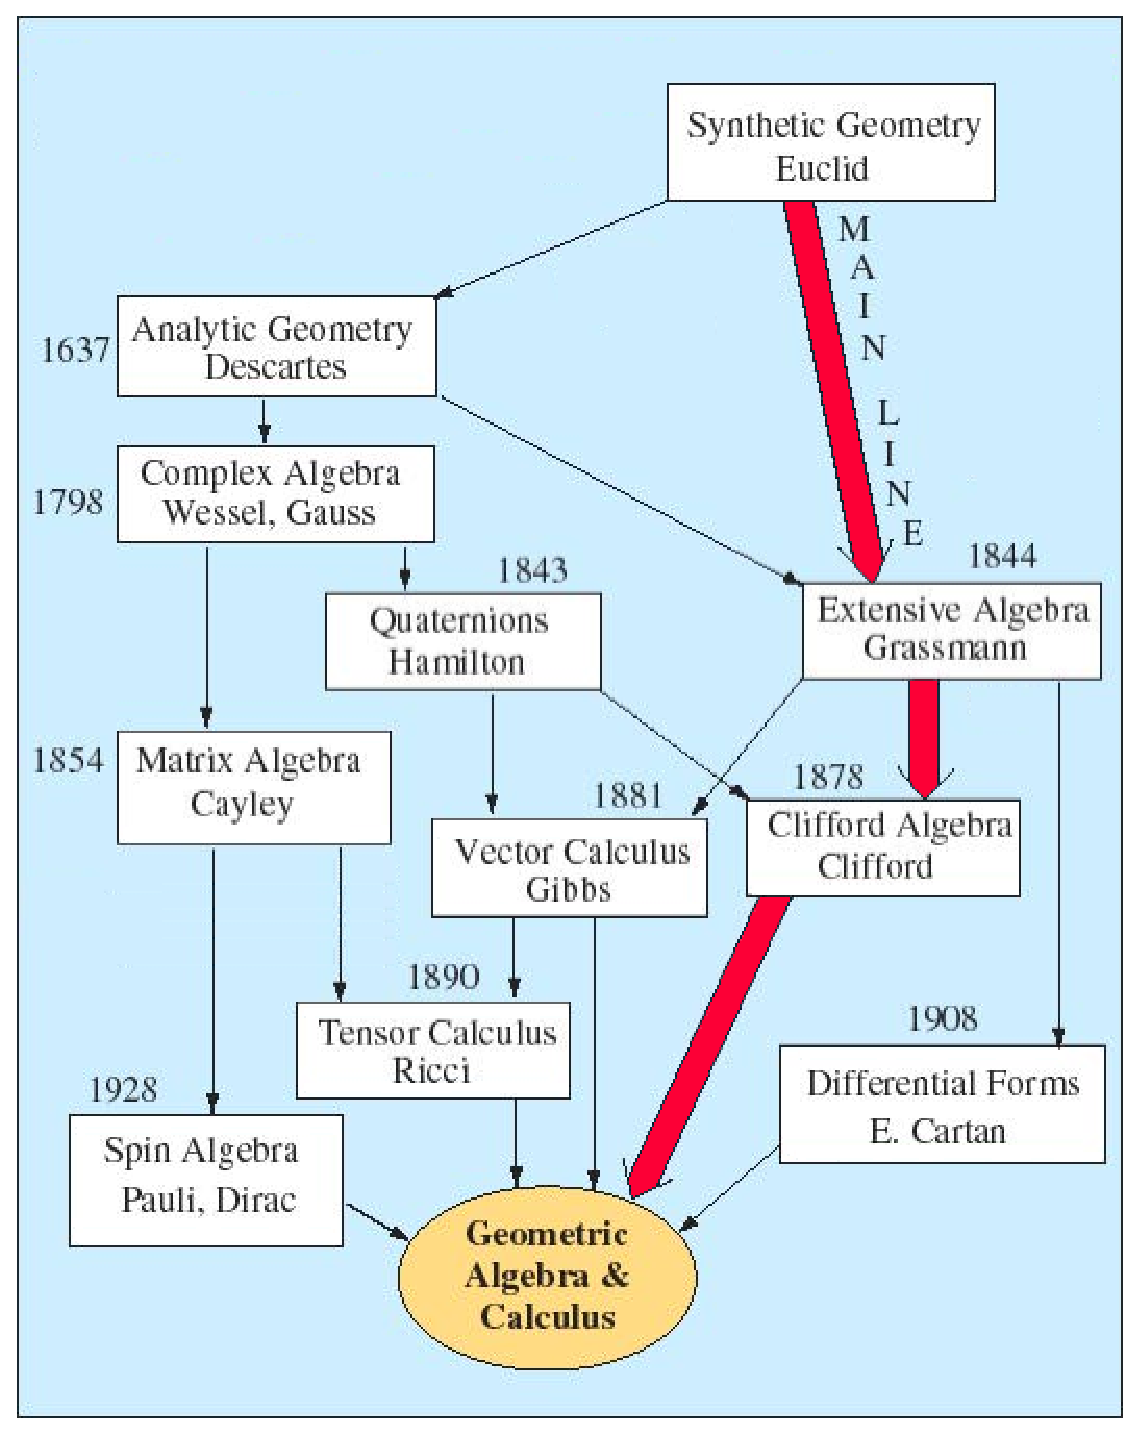
\includegraphics[scale=0.47]{DescentVectors}

\caption{\label{DescentOfVectors} The descent of the various vector systems. The main path of development beginning from Euclid geometry down through Grassman and then to Clifford. Other parallel developments using complex numbers, quaternions, Gibbs' vectors, tensors, matrices and spinor algebra subsumed into the general formalism of Clifford geometric algebra with the inclusion of calculus.}
\end{figure}
\end{center}

\end{frame}


%=========================================================================
\begin{frame}[fragile]{}

Most of the engineering EM analysis are performed in a three--dimensional space (3D). 
In the 3D space a very interesting fact takes place: \alert{GA is equivalent to Pauli algebra}.

Pauli matrices have been introduced by Wolfgang Pauli 
%(https://en.wikipedia.org/wiki/Wolfgang_Pauli) 
for the spin theory.

Very remarkably, \alert{by using Pauli matrices a vector can be represented as a 2x2 matrix}. 
Thus it is possible to multiply vectors by multiplying the relative matrices. 

\alert{It is also possible to make the inverse of a vector!}
\end{frame}

%=========================================================================
\begin{frame}[fragile]{GA in 3D and Pauli matrices}

In the 3D space, according to GA, we need to represent:
\alert{
\begin{itemize}
\item a scalar;
\item 3 vectors;
\item 3 bivectors;
\item psuedo--scalar
\end{itemize}
}
 i.e. 8 numbers. 

It is possible to introduce a \alert{multivector} which is the sum of a scalar, a vector, a bivector and a pseudo--scalar. 

Such multivector can be represented by a 2x2 matrix and can be constructed in terms of Pauli matrices. 

\end{frame}

%=========================================================================
\begin{frame}[shrink=25]{}

\begin{figure}[htb]
\begin{center}
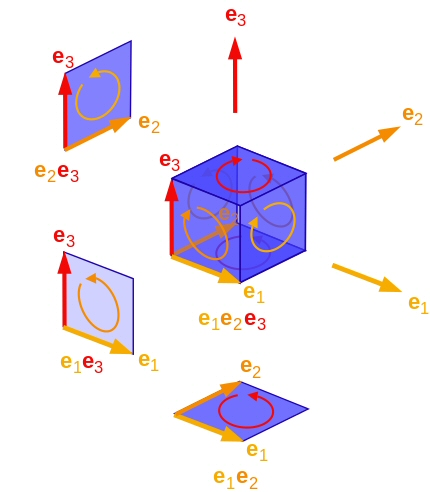
\includegraphics[width=3.5in]{GeometrySpace}
\end{center}
\caption{Identify the basis vectors as $e_1 = \sigma_1$, $e_2 = \sigma_2$, $e_3 = \sigma_3$.These are elements of Clifford's model for three--dimensional space. This consists of three unit vectors $ e_1, e_2 $ and $ e_3 $, three unit areas $ e_2 e_3, e_3 e_1 $ and $ e_1 e_2 $ and a unit volume $ \iGA = e_1 e_2 e_3 $. The pure scalars then defining points to form a complete algebraic description of three-dimensional physical space. \label{ThreeSpace}}
\end{figure}
\end{frame}
%=========================================================================
 \section{Pauli matrices and their properties}
 
 
%=========================================================================
\begin{frame}[shrink=10]{Wolfgang Pauli}
\begin{figure}[htb]

\begin{center}
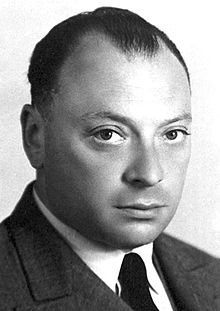
\includegraphics[width=1.0in]{220px-Pauli}
\end{center}

\caption{
Wolfgang Ernst Pauli (25 April 1900 -- 15 December 1958)
}

%https://en.wikipedia.org/wiki/Wolfgang_Pauli
\href{https://en.wikipedia.org/wiki/Wolfgang_Pauli}{\textcolor{blue}{Wolfgang Pauli}} was an Austrian-born Swiss and American theoretical physicist and one of the pioneers of quantum physics. 

In 1945, after having been nominated by Albert Einstein, Pauli received the Nobel Prize in Physics for his "decisive contribution through his discovery of a new law of Nature, the exclusion principle or Pauli principle". 

%The discovery involved spin theory, which is the basis of a theory of the structure of matter.
\end{figure}

\end{frame}


%=========================================================================
\begin{frame}[fragile]{Pauli matrices}



We first introduce the Pauli matrices and then discuss some of their properties and show how to operate with this new tool.

Note that \alert{engineers are quite well trained to operate with matrices} and we will see that many standard vectors operations can be simplified and new important elements will be found.

% The Pauli matrices are a set of three 2x2 complex matrices which are \emph{Hermitian} and \emph{unitary}. 
 
  The Pauli matrices have the following form
%
\begin{eqnarray}
\sigma_1 &= & \begin{pmatrix}0 & 1\cr 1 & 0\end{pmatrix} \nonumber \\
%
\sigma_2 &= & \begin{pmatrix}0 & -i\cr i & 0\end{pmatrix} \nonumber \\
%
\sigma_3 &= &\begin{pmatrix}1 & 0\cr 0 & -1\end{pmatrix}  \, .
%
\end{eqnarray}
%

\end{frame}

\begin{frame}[fragile]{Pauli matrices}
The Pauli matrices are a set of three 2x2 complex matrices which are \emph{Hermitian} and \emph{unitary}. 
 
 An \href{https://en.wikipedia.org/wiki/Hermitian_matrix}{\textcolor{blue}{Hermitian matrix}} (or \emph{self-adjoint} matrix) is a complex square matrix that is equal to its own conjugate transpose, that is, the element in the $i$-th row and $j$-th column is equal to the complex conjugate of the element in the $j$-th row and $i$-th column, for all indices $i$ and $j$.  Let us consider the matrix $a$
 %
\begin{eqnarray}
A &= & \begin{pmatrix}a_{11} & a_{12}\cr a_{21} & a_{22}\end{pmatrix} \nonumber
\end{eqnarray}
%
its transpose is given by
%
\begin{eqnarray}
A^T&= & \begin{pmatrix}a_{11} & a_{21}\cr a_{12} & a_{22}\end{pmatrix} \nonumber
\end{eqnarray}
%
\end{frame}
%=============================================================
\begin{frame}[fragile]{}
%

By denoting with $^*$ the complex conjugate, its Hermitian $A^\dag$ is
%
\begin{eqnarray}
A^\dag= & \begin{pmatrix}a_{11}^* & a_{21}^*\cr a_{12}^* & a_{22}^*\end{pmatrix} \nonumber
\end{eqnarray}
%
The \emph{trace} of $A$ is 
\be
tr(A) = a_{11}+a_{22} \, .
\ee

 A complex square matrix $U$ is unitary if its conjugate transpose $U^\dag$ is also its inverse.
 
\end{frame}
%=========================================================================
\begin{frame}[fragile]{Properties of the Pauli matrices}

It is immediately noted that the trace of these matrices is always zero. 

The determinant of the Pauli matrices is always -1.

The following products hold: 
%
\begin {equation}
\sigma_1^2 = \sigma_2^2 = \sigma_3^2 =  \begin{pmatrix}1 & 0\cr 0 & 1\end{pmatrix} = I = \sigma_0\,.
 \end{equation}
 %
By multiplying e.g. $\sigma_1$ with $\sigma_2$ the result is $i \sigma_3$ and similarly for the other cases:
%
\begin {eqnarray}
\sigma_1 \sigma_2 &=& i \sigma_3  = - \sigma_2 \sigma_1 \nonumber \\
\sigma_2 \sigma_3 &=& i \sigma_1 =  - \sigma_3  \sigma_2\nonumber \\
\sigma_3 \sigma_1 &=&  i \sigma_2 =  - \sigma_1  \sigma_3 \,.
\label{sigmacomb}
 \end{eqnarray}
 %

\end{frame}

%=========================================================================
\begin{frame}[fragile]{}
The above relations are very important. In fact, they show that, in the three-dimensional case, we can always replace the quantities $\sigma_i\sigma_j$ with the orthogonal vector $i \sigma_k$.
% (with the appropriate combination given in (\ref{sigmacomb})).
 
 From the above properties it is seen that
 \be\label{i123}
 (\sigma_1 \sigma_2 \sigma_3)^2 =  \sigma_1 \sigma_2 \sigma_3 \sigma_1 \sigma_2 \sigma_3 = -1 \
 \ee
i.e. $ \sigma_1 \sigma_2 \sigma_3 = i$.
 
The three Pauli matrices, with the addition of the identity matrix $\sigma_0$, form a basis in the space of the 2x2  Hermitian matrices and a matrix $A$ can be represented as:
%
\begin {equation}
A = a_0\sigma_0 + a_1 \sigma_1 + a_2 \sigma_2 + a_3 \sigma_3\,.
 \end{equation}
 %
It is worthwhile to note that when the coefficients ($a_0,a_1,a_2,a_3$) are complex, also non Hermitian matrices can be described by the basis of ($\sigma_0,\sigma_1,\sigma_2, \sigma_3$).

\end{frame}

%=========================================================================
\section{The Pauli vector}
%=========================================================================

%=========================================================================
\begin{frame}[fragile]{The Pauli vector}


Let us introduce the Pauli vector which is a vector made by the three matrices ($\sigma_1,\sigma_2, \sigma_3$).
%
\begin {equation}
{\bf \sigma} = \left(  \sigma_1 \, {\bf x}_0,  \sigma_2 \, {\bf y}_0 ,  \sigma_3\, {\bf z}_0  \right)\,.
 \end{equation}
 %
We can consider the vector $\Ba = \left(a_x\, {\bf x}_0 +  a_y \, {\bf y}_0 + a_z \, {\bf z}_0 \right)$  in the three-dimensional space and make the following product:
%%
%\begin {equation}
%\tilde{a} = {\bf \sigma} \cdot {\bf a} = 
%\sigma_1 a_x + \sigma_2 a_y +\sigma_3 a_z
%=\begin{pmatrix}a_z & a_x - i a_y \cr a_x + i a_y & -a_z\end{pmatrix}\,
%\label{Epauli}
% \end{equation}
% %
 %%%%%%%%%%%%%%%%%%%%%%%%%%%%%%%%%%%%%%%%%

\bea
\tilde{a} &=& {\bf \sigma} \cdot {\bf a} = 
\sigma_1 a_x + \sigma_2 a_y +\sigma_3 a_z \\
& = &  \begin{pmatrix}0 & 1\cr 1 & 0\end{pmatrix} a_x +
\begin{pmatrix}0 & -i\cr i & 0\end{pmatrix} a_y +
\begin{pmatrix}1 & 0\cr 0 & -1\end{pmatrix} a_z  \\
& = &
\begin{pmatrix}a_z & a_x - i a_y \cr a_x + i a_y & -a_z\end{pmatrix}\,
\label{Epauli}
\eea
 
 
% \be
%\tnabla   =   \sigma \cdot \nabla = \sigma_1 \partial_x + \sigma_2 \partial_y +\sigma_3 \partial_z  \nonumber
%\ee

The matrix $\tilde{a}$ is an equivalent description of the vector ${\bf a}$ in terms of a 2x2 matrix. Two different symbols have been used to denote the 2x2 matrix representation $\tilde{a}$  and the standard vector representation ${\bf a}$. 
%They refer to exactly the same quantity and it is always possible to pass from one to the other. 

\end{frame}

%=========================================================================
\begin{frame}[fragile]{Pauli matrices properties determination  with a computer algebra system}
%
\subsection{Pauli matrices properties determination  with a computer algebra system }

It is instructive to try to verify the properties previously illustrated by using a computer algebra system (CAS). Here following we use wxMaxima to define the 2x2 Pauli matrices and to perform some computations.
Please refer to the file:
\small
\begin{verbatim}
wxMaxima/Pauli_def.wxm
\end{verbatim}
\normalsize
%
which is listed in the following.



\end{frame}
%%=========================================================================
\begin{frame}[shrink=70]{Pauli definitions}
%
\small
\lstinputlisting{wxMaxima/Pauli_def.wxm}
\normalsize
\end{frame}
%=========================================================================
\begin{frame}[fragile]{Product }
%
We introduce the Pauli matrices and then the representation of two vectors $\Ba$ and $\Bb$ via their Pauli matrices $\ta,\tb$. Then we perform their product obtaining $\tc= \ta \tb$ as illustrated in the code :
%
\small
\begin{verbatim}
wxMaxima/Pauli_ab.wxm
\end{verbatim}
\normalsize
%
which is listed in the following.
\end{frame}

%=========================================================================
\begin{frame}[shrink=70]{}
%
\small
\lstinputlisting{wxMaxima/Pauli_ab.wxm}
\normalsize
\end{frame}





%=========================================================================
\begin{frame}[shrink=20]
Let us try the product between two matrices $\ta, \tb$ and evaluate their product $\tc = \ta \tb$,
\bea
\tiny
\ta & = & \begin{pmatrix}a_3 & a_1-i\,a_2\cr i\,a_2+a_1 & -a_3\end{pmatrix} \nonumber \\
\tb & = &\begin{pmatrix}b_3 & b_1-i\,b_2\cr i\,b_2+b_1 & -b_3\end{pmatrix} \nonumber \\
\tc & = &\begin{pmatrix}a_3\,b_3+\left( a_2+i\,a_1\right) \,b_2+\left( a_1-i\,a_2\right) \,b_1 & \left( i\,a_2-a_1\right) \,b_3-i\,a_3\,b_2+a_3\,b_1\cr \left( i\,a_2+a_1\right) \,b_3-i\,a_3\,b_2-a_3\,b_1 & a_3\,b_3+\left( a_2-i\,a_1\right) \,b_2+\left( i\,a_2+a_1\right) \,b_1\end{pmatrix} \nonumber
\normalsize
\eea
%

\begin{itemize}
\item \alert{\emph{the trace of $\tc=\ta \tb$ divided by 2 gives us the dot product}}.
\end{itemize}
\be \label{dotpauli}
\Ba \cdot \Bb = 
(\tc_{11} + \tc_{22})/2 = a_1\,b_1+a_2\,b_2+a_3\,b_3
\ee

It is straightforward to recognize that the component along $x,y, z$ can be easily retrieved by the following operations
%
\bea
c_x & = & \frac{{c}_{21}+{c}_{12}}{2} \nonumber \\
c_y & = &  -\frac{i\,\left( {c}_{21}-{c}_{12}\right) }{2}\nonumber \\
c_z & = &  \frac{{c}_{11}-{c}_{22}}{2}
\eea
%

\end{frame}


%=========================================================================
\begin{frame}[shrink=20]

By writing them explicitly we find:
%
\bea
c_x & = & i\,\left( a_2\,b_3-a_3\,b_2\right)  \nonumber \\
c_y & = &  -i\,\left( a_1\,b_3-a_3\,b_1\right)  \nonumber \\
c_z & = &  i\,\left( a_1\,b_2-a_2\,b_1\right) 
\eea
%
It is now easy to recognize that, apart for the $i$ factor, this  is equal to the well known cross product.
This new part is called \alert{ \emph{external product} and is denoted by $\Ba \wedge \Bb$}. We have just obtained the important identity:
%
\be \label{epcross}
\Ba \wedge \Bb = i \, \Ba \times \Bb \, .
\ee
%
Naturally, to represent the wedge product in terms of the Pauli matrices it is sufficient to subtract the dot product from $\ta \tb$, thus obtaining
%
\be \label{epcrossexplicit}
\Ba \wedge \Bb = \begin{pmatrix}i\,\left( a_1\,b_2-a_2\,b_1\right)  & i\,a_2\,b_3-a_1\,b_3-i\,a_3\,b_2+a_3\,b_1\cr i\,a_2\,b_3+a_1\,b_3-i\,a_3\,b_2-a_3\,b_1 & -i\,\left( a_1\,b_2-a_2\,b_1\right) \end{pmatrix} \, .
\ee
%
The quantity \alert{$\Ba \wedge \Bb$ is  a  \emph{bivector}} . 
\end{frame}







%=============================================================
\begin{frame}[fragile]{The product $\tb \ta$}
\subsection{The product $\tb \ta$}

It is immediate, by applying the rules of matrix multiplication, to compute the product $\tb \ta$. An example of code doing this is reported in:
%
\small
\begin{verbatim}
wxMaxima/Pauli_ba.wxm
\end{verbatim}
\normalsize
%
which is listed in the following.

\end{frame}
%=========================================================================
\begin{frame}[shrink=70]{$\tb, \ta$}
\small
\lstinputlisting{wxMaxima/Pauli_ba.wxm}
\normalsize
\end{frame}
%=========================================================================
\begin{frame}[shrink=30]{$\tb, \ta$}
Naturally, the Pauli matrices and the matrices $\ta, \tb$ are the same as before. However, now we have:
%
\bea
\td & = &  \tb \ta =
\begin{pmatrix}a_3\,b_3+\left( a_2-i\,a_1\right) \,b_2+\left( i\,a_2+a_1\right) \,b_1 & \left( a_1-i\,a_2\right) \,b_3+i\,a_3\,b_2-a_3\,b_1\cr \left( -i\,a_2-a_1\right) \,b_3+i\,a_3\,b_2+a_3\,b_1 & a_3\,b_3+\left( a_2+i\,a_1\right) \,b_2+\left( a_1-i\,a_2\right) \,b_1\end{pmatrix} \nonumber
\eea
%

It is apparent that the trace is the same as the one from $\ta \tb$.

By writing  explicitly the various components we find:
%
\bea
d_x & = & -i\,\left( a_2\,b_3-a_3\,b_2\right)  \nonumber \\
d_y & = & i\,\left( a_1\,b_3-a_3\,b_1\right)   \nonumber \\
d_z & = &  -i\,\left( a_1\,b_2-a_2\,b_1\right) 
\eea
%

\end{frame}
%=========================================================================
\begin{frame}[fragile]{Relation between cross and external product}

It is now easy to recognize that these  are the coefficient of $-i \, \Ba \times \Bb$.
The \emph{external product}  $\Bb \wedge \Ba$ thus satisfy the rule:
%
\be \label{epcross3}
\Bb \wedge \Ba = - \Ba \wedge \Bb = -i \, \Ba \times \Bb \, .
\ee
%

We have another relevant property: \alert{\emph{the external product between two vectors is anti--commutative}}. 
\end{frame}
%
%=============================================================
\begin{frame}[fragile]{Alternative definitions}


We have therefore found that the dot product can also be obtained as: 
%
\be \label{intdef}
\Ba \cdot \Bb = \frac{\ta \tb + \tb \ta}{2} \, ,
\ee
%
while for the external product we have:
%
\be \label{extdef}
\Ba \wedge \Bb = \frac{\ta \tb - \tb \ta}{2} \, .
\ee
%
The relations (\ref{intdef}), (\ref{extdef}) can be also taken as the definitions of dot and external products, respectively.
\end{frame}

%=========================================================================
%\begin{frame}[fragile]{}
%
%\end{frame}
%%=========================================================================
%\begin{frame}[fragile]{}
%
%\end{frame}
%


%=============================================================
\begin{frame}[fragile]{Inner product}
%
\subsubsection{Inner product}
The inner product between two matrices $A$ and $B$ can be defined as following
\be
\left<A,B\right> = \frac{1}{2} tr \, (AB^\dag) \, .
\ee
%
From the properties of the Pauli matrices it is readily recognized that, for $i \ne j$ we have $\left<\sigma_i,\sigma_j\right>=0$, while $\left<\sigma_i,\sigma_i\right>=1$.
This provides a simple way to retrieve the coefficients of the Pauli matrices for a given matrix $A$.
In fact, we have
\bea
\left<A,\sigma_0\right> & = & a_0 \left<\sigma_0,\sigma_0\right> +  a_1 \left<\sigma_1,\sigma_0\right>
+ a_2 \left<\sigma_2,\sigma_0\right> +  a_3 \left<\sigma_3,\sigma_0\right> = a_0 \nonumber
\eea
and similarly for other components.

\end{frame}


%=========================================================================
\begin{frame}[fragile]{}
Once we have represented the vector $\Ba$ as a matrix $\ta$ it is possible to compute its determinant and its inverse.

It is immediately recognized that we have for the determinant
%
\be \label{deta}
det(\ta) =  -(a_1^2 + a_2^2 + a_3^2)\, 
\ee
%
from which it is evident that, \alert{by taking the square root of the absolute value, we can recover the modulus of the vector}.
%

In standard vector algebra \alert{the inverse of a vector} is not defined. However we can perform the inverse of $\ta$ obtaining
%
\be \label{inva}
\ta^{-1} =\frac{1}{{a_1}^{2}+{a_2}^{2}+{a_3}^{2}} \begin{pmatrix}a_3 & -i\,a_2+a_1\cr i\,a_2+a_1 & -a_3\end{pmatrix}\, 
\ee
%
This is just the same vector divided by the square of its modulus!


\end{frame}

%=========================================================================
\begin{frame}[fragile]{Finding the operator which transforms one vector into another}
\subsection{Finding the operator which transforms one vector into another}
Let us assume that the vectors $\Ba, \Bb$ are given and we want to find the operator that transforms vector $\Ba$ into vector $\Bb$.

In conventional vector analysis, apart for particular cases, this is not a simple operation. 

Using Pauli matrices it is quite trivial. In fact, by calling with $\tc$ the transformation we have that
\be
\tb = \tc \ta
\ee

The transformation is simply
\be
\tc = \tb \ta^{-1}\,.
\ee

\end{frame}

%%=============================================================
\begin{frame}[fragile]{Triple products with Pauli matrices}
%
\subsection{Triple products with Pauli matrices}

Let us now investigate the \alert{triple product}. 

We start by considering the product $\Ba  (\Bb \wedge \Bc)$ and by expressing $\Bb \wedge \Bc$. 

In (\ref{epcrossexplicit}) the geometric product has been written for $\Ba \wedge \Bb$ and it is now repeated giving:

%
\be \label{bwc}
\Bb \wedge  \Bc =  
\begin{pmatrix}i\,b_1\,c_2-i\,b_2\,c_1 & \left( i\,b_2-b_1\right) \,c_3-i\,b_3\,c_2+b_3\,c_1\cr
 \left( i\,b_2+b_1\right) \,c_3-i\,b_3\,c_2-b_3\,c_1 & i\,b_2\,c_1-i\,b_1\,c_2\end{pmatrix} \, .
\ee
%

\end{frame}
%%=========================================================================
\begin{frame}[fragile]{}
%
The next step is to obtain $d = \Ba(\Bb \wedge \Bc)$ which simply reduces to the matrix multiplication of $\Ba$ and $\Bb \wedge \Bc$.

This operation, together with a few others is reported in the following code. 

Note that we have used the symbol $d$ to denote the result but we still need to identify what type of result we are going to get.

 It will be a 2x2 matrix but the meaning of its components is still to be found. Please refer to the following code as an example:
 %
\small
\begin{verbatim}
wxMaxima/Pauli_abc.wxm
\end{verbatim}
\normalsize
%


\end{frame}
%%=========================================================================
\begin{frame}[shrink=70]{triple product}
%

\small
\lstinputlisting{wxMaxima/Pauli_abc.wxm}
\normalsize

\end{frame}
%%=========================================================================
\begin{frame}[shrink=30]{Scalar part}
%
After performing the matrix multiplication one get
%
\bea \label{abwc}
d & = & \Ba(\Bb \wedge \Bc)  \\
d_{11} & = &   \left( a_1-i\,a_2\right) \,\left( \left( i\,b_2+b_1\right) \,c_3-i\,b_3\,c_2-b_3\,c_1\right) +a_3\,\left( i\,b_1\,c_2-i\,b_2\,c_1\right)  \nonumber \\
d_{12} & = &  a_3\,\left( \left( i\,b_2-b_1\right) \,c_3-i\,b_3\,c_2+b_3\,c_1\right) +\left( a_1-i\,a_2\right) \,\left( i\,b_2\,c_1-i\,b_1\,c_2\right) \nonumber \\
d_{21} & = &  \left( i\,a_2+a_1\right) \,\left( i\,b_1\,c_2-i\,b_2\,c_1\right) -a_3\,\left( \left( i\,b_2+b_1\right) \,c_3-i\,b_3\,c_2-b_3\,c_1\right) \nonumber \\
d_{22} & = & \left( i\,a_2+a_1\right) \,\left( \left( i\,b_2-b_1\right) \,c_3-i\,b_3\,c_2+b_3\,c_1\right) -a_3\,\left( i\,b_2\,c_1-i\,b_1\,c_2\right)  \nonumber 
\eea
%
\subsubsection{Scalar part}
As before the scalar part of $d$ is obtained by taking half of the trace and is denoted here (for reasons that will become clear in the following) as 
$\left< d\right>_3$
%
\be \label{d_3}
\left< d\right>_3 = i\,\left( a_1\,b_2\,c_3-a_2\,b_1\,c_3-a_1\,b_3\,c_2+a_3\,b_1\,c_2+a_2\,b_3\,c_1-a_3\,b_2\,c_1\right) 
\ee
%
\alert{It is noted that there is the factor $i$ in front of the expression}. 

This part corresponds to a \alert{\emph{trivector}}, i.e. to the volume element obtained by performing
$\Ba \wedge \Bb \wedge \Bc$.
\end{frame}
%
%%=============================================================
\begin{frame}[fragile]{pseudoscalar}
%
It is also observed that if we consider the matrix
\be
abc = \begin{pmatrix}a_1 & a_2 & a_3\cr b_1 & b_2 & b_3\cr c_1 & c_2 & c_3\end{pmatrix}
\ee
its determinant is 
\be \label{detabc}
det(abc) = a_1\,\left( b_2\,c_3-b_3\,c_2\right) -a_2\,\left( b_1\,c_3-b_3\,c_1\right) +a_3\,\left( b_1\,c_2-b_2\,c_1\right) 
\ee
%
and, when multiplied by $i$ coincides with (\ref{d_3}). We have therefore derived the important property:
\be \label{awbwc}
\Ba \wedge \Bb \wedge \Bc = i \, det \, (abc) = \left< d\right>_3
\ee
It is noted that \alert{$\Ba \wedge \Bb \wedge \Bc$ is often called \emph{pseudoscalar}} i.e. is a scalar quantity multiplied by $i$.
In the 3D space this is the element of the third grade (this is the reason why we have used $\left< d\right>_3)$. This is also the highest grade in 3D.
\end{frame}
%=========================================================================
\begin{frame}[fragile]{observations}
%
A few observations are in order:
\bea 
(\Ba \wedge \Bb) \wedge \Bc & = & \Ba \wedge (\Bb \wedge \Bc) \label{ppp} \\
\Ba \wedge \Bb \wedge \Bc \wedge \Bd & = & 0 \label{abcd0}
\eea
%

In (\ref{ppp}) it is noted that, \emph{unlikely to the cross product}, \alert{the wedge product can be computed without a particular order}.

The other property in (\ref{abcd0}) tell us the following. If we have assumed that the \alert{three vectors $\Ba, \Bb, \Bc$ span the 3D space (i.e. they do not lay on a plane, than a vector $\Bd$ cannot be external to them}, i.e. its external part is zero.

\end{frame}
%%=========================================================================
\begin{frame}[fragile]{Bivectors}
%
Let us introduce the \alert{bivector $\hat{\BB} = \Bb \wedge \Bc$}. It is apparent that we have that \alert{\emph{the external product between a vector and a bivector is commutative}}:
\be
\Ba \wedge \hat{\BB} = \hat{\BB} \wedge \Ba \, .
\ee

\subsubsection{Vector part $\Ba \cdot (\Bb \wedge \Bc)$ }
Once from the matrix  $d$ in (\ref{abwc}) the scalar part is removed, the remaining part corresponds to $\Bw = \Ba \cdot (\Bb \wedge \Bc)$. If we express the components relative to this matrix we have:
%
\bea 
w_{x} & = &  -a_3\,b_1\,c_3-a_2\,b_1\,c_2+\left( a_3\,b_3+a_2\,b_2\right) \,c_1 \nonumber \\
w_{y} & = &  -a_3\,b_2\,c_3+\left( a_3\,b_3+a_1\,b_1\right) \,c_2-a_1\,b_2\,c_1 \nonumber \\
w_{z} & = & \left( a_2\,b_2+a_1\,b_1\right) \,c_3-a_2\,b_3\,c_2-a_1\,b_3\,c_1  \label{adotbwc} 
\eea
%
it is noted that they are the same coefficients, apart for a sign, that we would have obtained by performing the vector product $\Bv = \Ba \times \Bb \times \Bc$.
\end{frame}
%%=========================================================================
\begin{frame}[fragile]{$\Ba \cdot \Bb \wedge \Bc = - \Ba \times \Bb \times \Bc$}
%
In fact,
in the last part of the code, we perform the triple vector product obtaining:
%
\bea 
v_{x} & = &  a_3\,b_1\,c_3+a_2\,b_1\,c_2+\left( -a_3\,b_3-a_2\,b_2\right) \,c_1 \nonumber \\
v_{y} & = &  a_3\,b_2\,c_3+\left( -a_3\,b_3-a_1\,b_1\right) \,c_2+a_1\,b_2\,c_1 \nonumber \\
v_{z} & = & \left( -a_2\,b_2-a_1\,b_1\right) \,c_3+a_2\,b_3\,c_2+a_1\,b_3\,c_1 \label{atbtc}  \, .
\eea
%
By comparing (\ref{atbtc}) with (\ref{adotbwc}) it is readily recognized that we have found another important relationship i.e.
%
\be \label{adbwcatbtc}
\Ba \cdot \Bb \wedge \Bc = - \Ba \times \Bb \times \Bc
\ee
\end{frame}
%
%=========================================================================
\begin{frame}[fragile]{$ 
\Ba \cdot \Bb \wedge \Bc = - \Ba \times \Bb \times \Bc = ({\bf a}  \cdot  {\bf b})    {\bf c} - ({\bf a}  \cdot  {\bf c})  {\bf b}
$}
%
In passing, it is reminded that we have already introduced the relationship 
${\bf a} \times ( {\bf b} \times  {\bf c})  =   ({\bf a}  \cdot  {\bf c})  {\bf b} -  ({\bf a}  \cdot  {\bf b})    {\bf c}$.

We can also compute $\Ba \cdot \Bb \wedge \Bc$ as
%
\be \label{adbwcatbtcc}
\Ba \cdot \Bb \wedge \Bc = - \Ba \times \Bb \times \Bc = ({\bf a}  \cdot  {\bf b})    {\bf c} - ({\bf a}  \cdot  {\bf c})  {\bf b}
\ee
%
This computation is also performed in the code, where the dot products are obtained as e.g. $\Ba \cdot \Bb = \left( \ta \tb + \tb \ta \right)/2$ and then proceeding with standard matrix multiplication.
\end{frame}
%%=========================================================================
\begin{frame}[fragile]{}
%
So far we have considered the external product of a bivector with a vector (or viceversa) and we have obtained a trivector. 

Then we have considered the dot product of a vector with a bivector, obtaining a vector. 

It is thus natural to pose the question: what is the result  of a product of the type 
$ \Bb \wedge \Bc  \cdot \Ba$? 

In other words, the dot product of a \emph{bivector} with a vector is commutative or anticommutative?
In order to answer to this question we can consider the following code.

\small
\begin{verbatim}
wxMaxima/Pauli_bca.wxm
\end{verbatim}
\normalsize
%
which is listed in the following.



\end{frame}
%%=========================================================================
\begin{frame}[shrink=70]{}
%
\small
\lstinputlisting{wxMaxima/Pauli_bca.wxm}
\normalsize
\end{frame}
%

\begin{frame}[fragile]{the dot product for bivectors is anticommutative}
The initial part is identical as before, the difference only coming out when we compute
$ (\Bb \wedge \Bc) \Ba$. 

The result is a 2x2 matrix with half of the trace that now corresponds to 
$ \Bb \wedge \Bc  \wedge \Ba $.

We thus have $ \Bb \wedge \Bc  \wedge \Ba = \Ba \wedge \Bb \wedge \Bc$. 

By subtracting this part (times $\sigma_0$) from the matrix $ (\Bb \wedge \Bc) \Ba$
we obtain the matrix representing $ (\Bb \wedge \Bc) \cdot \Ba$ with the components which are the same as in (\ref{adotbwc}) but with a minus sign.

\alert{Therefore, \emph{the dot product for bivectors is anticommutative}} or 
%
\be \label{bidotanti}
\Ba \cdot \Bb \wedge \Bc = - \Bb \wedge \Bc \cdot \Ba \, .
\ee
\end{frame}

%%=============================================================
\begin{frame}[fragile]{Bivectors dot and wedge products}
Therefore for a bivector $\hat{\BB}$ we can write
%
\bea
\Ba \cdot \hat{\BB} & = & \frac{1}{2}\left(\Ba \hat{\BB} - \hat{\BB} \Ba \right) = - \Ba \times \Bb \times \Bc  \label{atbtc2}\\
\Ba \wedge \hat{\BB} & = & \frac{1}{2}\left(\Ba \hat{\BB} + \hat{\BB} \Ba \right) =  \Ba \cdot \left( \Bb \times \Bc\right) \,  i  \label{adbtc2}
\eea

The last equality has not been shown so far, but the reader can easily prove it.
\end{frame}
%%=============================================================
\begin{frame}[fragile]{the vector $\BB=\Bb \times \Bc $}
By introducing the vector $\BB=\Bb \times \Bc $ we have
\be \label{vbv}
\hat{\BB} =  \Bb \wedge \Bc = i \, \Bb \times \Bc = i \, \BB
\ee
which, by using (\ref{atbtc2}, \ref{adbtc2}), allows to write
%%
\bea
\Ba \cdot \hat{\BB} & = &  - \Ba \times \BB  \label{atbtcm}\\
\Ba \wedge \hat{\BB} & = &   \Ba \cdot  \BB  \,  i  \label{adbtcm}
\eea
%
\end{frame}
%%=============================================================
\begin{frame}[fragile]{Relating classical vector analysis with the Pauli algebra}
\alert{Equation (\ref{vbv}) shows that a bivector $\hat{\BB} $ can be obtained from a vector $\BB$ simply by multiplication times $i$ (and viceversa)}.
 
It is also noted that a scalar $t$ when multiplied by $i$ becomes a trivector (and viceversa).

The relationships (\ref{atbtcm}, \ref{adbtcm}) can be used for \alert{relating classical vector analysis with the Pauli algebra}. 
\end{frame}

%%%=============================================================
%%\begin{frame}[fragile]{}
%%\end{frame}
%%%=============================================================

%=========================================================================
\section{Vector analysis with Pauli matrices (summary)}
%=========================================================================

%=========================================================================
\begin{frame}[fragile]{Vector analysis with Pauli matrices}
%\subsection{Short summary of the results of vector analysis with Pauli matrices}
\begin{itemize}
\item Three--dimensional vectors can be represented using 2x2 Pauli matrices.
%
\begin {equation}
\tilde{a} =  \begin{pmatrix}a_z & a_x - i a_y \cr a_x + i a_y & -a_z\end{pmatrix}\,
\label{Epauli}
 \end{equation}
 %
\item Multiplication of two matrices corresponding to two vectors give us both the dot product and another new part, the external product. \alert{This multiplication corresponds to the geometric or Clifford product.
%
\be \label{funids}
\Ba  \Bb =  \Ba \cdot \Bb + \Ba \wedge \Bb \, = \ta \tb.
\ee
%
}
\end{itemize}
\end{frame}

\begin{frame}[fragile]{Vector analysis with Pauli matrices}
%\subsection{Short summary of the results of vector analysis with Pauli matrices}
\begin{itemize}
\item \alert{dot product} between two vectors \alert{is commutative}: 
%
\be \label{intdef}
\Ba \cdot \Bb = \Bb \cdot \Ba = \frac{\ta \tb + \tb \ta}{2} \, ,
\ee
%
\item \alert{the external product} between two vectors \alert{is anticommutative}
%
\be \label{extdef}
\Ba \wedge \Bb = - \Bb \wedge \Ba =\frac{\ta \tb - \tb \ta}{2} \, .
\ee
%
\item the external product, in 3D, is related to the cross product as:
%
\be \label{epcross3}
\Ba \wedge \Bb =  i \, \Ba \times \Bb \, .
\ee
%
\end{itemize}

\end{frame}

%=========================================================================
\begin{frame}[fragile]{}
\begin{itemize}
\item the external product between two vectors introduces a new subject:  \emph{the bivector}.
\item the bivector can be expressed either showing the two vector components or a single vector component but multiplied by $i$ 
%
\begin {eqnarray}
\sigma_1 \sigma_2 &=& i \sigma_3  = - \sigma_2 \sigma_1 \nonumber \\
\sigma_2 \sigma_3 &=& i \sigma_1 =  - \sigma_3  \sigma_2\nonumber \\
\sigma_3 \sigma_1 &=&  i \sigma_2 =  - \sigma_1  \sigma_3 \,.
\label{sigmacomb}
 \end{eqnarray}
 %
\item 
A bivector $\hat{\BB} = \Bb \wedge \Bc$ can be multiplied by a vector giving rise to a vector and a \emph{trivector}:
\be \label{aB}
\Ba \, \hat{\BB} = \Ba \cdot \hat{\BB} + \Ba \wedge \hat{\BB}
\ee
\end{itemize}

\end{frame}

%=========================================================================

\begin{frame}[fragile]{}
\begin{itemize}

\item the internal product of a vector with a bivector is given by
\be 
\Ba \cdot \hat{\BB}  =  \frac{1}{2}\left(\Ba \hat{\BB} - \hat{\BB} \Ba \right) = - \Ba \times \Bb \times \Bc = - \Ba \times \BB
\ee
\item the external product of a vector and a bivector is
%
\be 
\Ba \wedge \hat{\BB}  =  \frac{1}{2}\left(\Ba \hat{\BB} + \hat{\BB} \Ba \right) =  \Ba \cdot \left( \Bb \times \Bc\right) \,  i  =  \Ba \cdot  \BB  \,  i 
\ee

\item the dot product of a vector and a bivector is anticommutative and it is related to the cross product as:
\be \label{adbwcatbtccs}
\Ba \cdot \Bb \wedge \Bc = - \Ba \times \Bb \times \Bc = ({\bf a}  \cdot  {\bf b})    {\bf c} - ({\bf a}  \cdot  {\bf c})  {\bf b} = -\Bb \wedge \Bc \cdot \Ba
\ee

\end{itemize}

\end{frame}

%=========================================================================
\begin{frame}[fragile]{Space description}


%\subsubsection{Space description}
It is noted that elements  three-dimensional space are described by eight numbers (i.e. a complex 2x2 matrix). In particular they are: 
\begin{itemize}
\item one \emph{scalar} ($\sigma_0$). Grade $0$
\item 3 basis \emph{vectors} ($\sigma_1, \sigma_2, \sigma_3$) i.e. three directions. Grade $1$
\item 3 basis \emph{bivectors} ($\sigma_1 \sigma_2, \sigma_1 \sigma_3, \sigma_2 \sigma_3$). Grade $2$
\item one \emph{pseudoscalar} ($\sigma_1 \, \sigma_2 \, \sigma_3$). Grade $3$
\end{itemize}
%
All these elements are contained in a 2x2 matrix and, similarly to what we do for complex numbers, they can be written together in a 
\alert{ \emph{multivector} $\mathit{M}$} as
\be \label{Mmultivector}
\mathit{M} = 
a_0 + \, \Ba + \, \hat{\BB} +  \hat{\mathit{t}}
\ee
where $a_0$ is a scalar, $\Ba$ is a vector, $\hat{\BB}$ is a bivector and $\hat{\mathit{t}}$ is a pseudoscalar.

\end{frame}

%=========================================================================
%\begin{frame}[shrink=10]{Multivector}
\begin{frame}[fragile]{Multivector}

\begin{figure}[htb]

\begin{center}
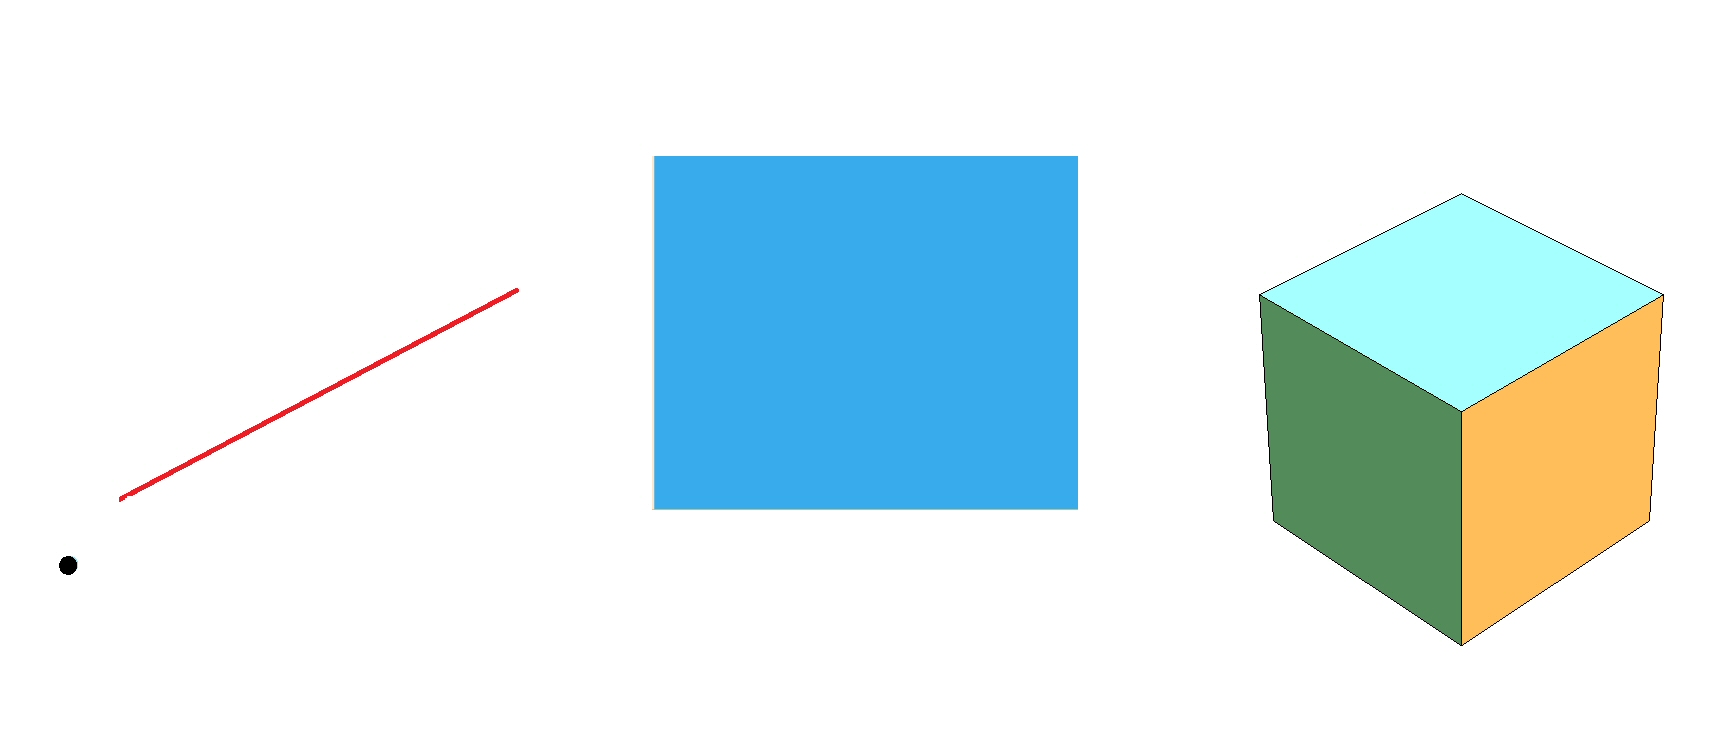
\includegraphics[width=3.4in]{Multi}
\end{center}

\caption{A multivector $\mathit{M} = 
a_0 + \, \Ba + \, \hat{\BB} +  \hat{\mathit{t}}$ representing a point, line, area and volume, that can be added, subtracted, multiplied or divided by other multivectors. \label{MultiPic}}

\end{figure}


\end{frame}

%=========================================================================
\begin{frame}[fragile]{Pauli matrix representation of a multivvector}

%\subsection{Pauli matrix representation of a multivvector}
\small
Let us see with more details the Pauli matrix representation of a multivector. The corresponding matrices of the multivector in (\ref{Mmultivector}) are given next:
%

\bea
\tilde{a_0} & = & \begin{pmatrix}a_0 & 0\cr 0 & a_0\end{pmatrix} \nonumber \\
\ta & = & \begin{pmatrix}a_3 & a_1-i\,a_2\cr i\,a_2+a_1 & -a_3\end{pmatrix} \nonumber \\
\tilde{B} & = & \begin{pmatrix}i\,B_3 & B_2+i\,B_1\cr i\,B_1-B_2 & -i\,B_3\end{pmatrix} \nonumber \\
\tilde{t} & = & \begin{pmatrix}i\,t & 0\cr 0 & i\,t\end{pmatrix} \label{Paulimult} \, .
 \eea
%
The matrices in (\ref{Paulimult}) can be summed together giving for  the multivector $\mathit{M}$
\be \label{Mmultivector:10}
\tilde{\mathit{M} }= 
\begin{pmatrix}i\,B_3+i\,t+a_3+a_0 & B_2+i\,B_1-i\,a_2+a_1\cr -B_2+i\,B_1+i\,a_2+a_1 & -i\,B_3+i\,t-a_3+a_0\end{pmatrix} \, .
\ee
%
Naturally, for a given Pauli matrix, it is straightforward to retrieve the elements of the different grades.
%
\normalsize

\end{frame}

%=========================================================================
\begin{frame}[shrink=20]{}

\subsection{Retrieving the elements of a multivector}
Let us assume that the matrix in (\ref{Mmultivector:10}) is given and we want to retrieve the various elements.
It is convenient to extract the real and imaginary part of $\tilde{\mathit{M} }$ as
%
\bea
\tilde{M_r} & = & \Re{\tilde{\mathit{M} }} = \begin{pmatrix}a_3+a_0 & B_2+a_1\cr a_1-B_2 & a_0-a_3\end{pmatrix}\nonumber \\
\tilde{M_i} & = & \Im{\tilde{\mathit{M} }} =  \begin{pmatrix}B_3+t & B_1-a_2\cr B_1+a_2 & t-B_3\end{pmatrix} \, . \label{Mmultivector:20}
 \eea
 %
By inspection, it is seen that we have the following identities:
%
\bea
a_0 & = & \frac{1}{2} \left(  \tilde{M_r}_{11} +  \tilde{M_r}_{22} \right)  \nonumber \\
a_1 & = & \frac{1}{2} \left(  \tilde{M_r}_{12} +  \tilde{M_r}_{21} \right)  \nonumber \\
a_2 & = & \frac{1}{2} \left(  \tilde{M_i}_{21}  -  \tilde{M_i}_{12} \right)  \nonumber \\
a_3 & = & \frac{1}{2} \left(  \tilde{M_r}_{11}  -  \tilde{M_r}_{22} \right)  \nonumber \\
B_1 & = & \frac{1}{2} \left(  \tilde{M_i}_{21}  +  \tilde{M_i}_{12} \right)  \nonumber \\
B_2 & = & \frac{1}{2} \left(  \tilde{M_r}_{12} -  \tilde{M_r}_{21} \right)  \nonumber \\
B_3 & = & \frac{1}{2} \left(  \tilde{M_i}_{11}  -  \tilde{M_i}_{22} \right)  \nonumber \\
t & = & \frac{1}{2} \left(  \tilde{M_i}_{11}  +  \tilde{M_i}_{22} \right)
 \, . \label{Mmultivector:30}
 \eea
 %
\end{frame}

%

%%=============================================================
\begin{frame}[shrink=70]{}
%
The code for converting multivectors into their Pauli matrix equivalent and viceversa is given in the following lines.

\small
\lstinputlisting{wxMaxima/Pauli_multivectors.wxm}
\normalsize
\end{frame}
%%=========================================================================
%\begin{frame}[fragile]{}
%
%\end{frame}
%%=========================================================================
%\begin{frame}[fragile]{}
%
%\end{frame}
%%=========================================================================
%\begin{frame}[fragile]{}
%
%\end{frame}
%




\end{document}
